\documentclass[a4paper, 11pt]{article}   	
\usepackage{geometry}       
\geometry{a4paper}
\geometry{margin=1in}	
\usepackage{paralist}
  \let\itemize\compactitem
  \let\enditemize\endcompactitem
  \let\enumerate\compactenum
  \let\endenumerate\endcompactenum
  \let\description\compactdesc
  \let\enddescription\endcompactdesc
  \pltopsep=\medskipamount
  \plitemsep=1pt
  \plparsep=1pt
\usepackage[english]{babel}

%/////////////////////////////////////////////////////////////////////////////
% math pkgs
\usepackage{bbm, bm, amsmath, amssymb, amsthm, mathrsfs, booktabs}
\theoremstyle{definition}
\newtheorem{theorem}{Theorem}
\newtheorem{lemma}{Lemma}
\newtheorem{corollary}{Corollary}
\newtheorem{definition}{Definition}
\newtheorem{proposition}{Proposition}
\newtheorem{procedure}{Procedure}
\newtheorem{construction}{Construction}
\newtheorem{example}{Example}
\newtheorem{remark}{Remark}
\newtheorem{claim}{Claim}
%/////////////////////////////////////////////////////////////////////////////
% tikz
\usepackage{tikz}
\usetikzlibrary{arrows}
\usepackage{poker_slide}


%/////////////////////////////////////////////////////////////////////////////
%/////////////////////////////////////////////////////////////////////////////

\title{\textbf{A Research on Card Shuffling and MCMC Paradigm} \\ Stochastic Process (2016) Course Project}
\author{CHEN, You; WANG, Shu; YANG, Ze; FENG, Biaojian}

\begin{document}
\maketitle
\section{Introduction}
\textit{This project is inspired by course 6.896, 2011 Spring in MIT.}\cite{mit} 
This project aims to study the theory and implementation of \textit{Markov Chain Monte Carlo} algorithm. We discuss general MCMC paradigm through the famous card-shuffling problem arisen in combinatorics. We will model the card shuffle by markov chain, and further discuss its stationary distribution, viariation distance and mixing time. Numerical computations will also be performed to validate the theory.

%/////////////////////////////////////////////////////////////////////////////
\section{Illustration of the Problam and Related Theories}
%/////////////////////////////////////////////////////////////////////////////
\subsection{The MCMC Paradigm} 
Consider probability space $(\Omega, \mathcal{F}, \mathbb{P})$. We define a real, positive \textit{weight function} $w:\Omega \to \mathbb{R}^+$. The goal is to sample an element $x\in\Omega$, with probability distribution $\pi(x)=\mathbb{P}\left(X=x\right)$ defined as
$$\pi(x):=\frac{w(x)}{Z_w};~~Z_w:=\sum_{x\in\Omega}w(x)$$
Where $Z_w$ is called the partition function of weight function $w$ in Omega. \\
In MCMC paradigm, we establish a general iterative solution approach to this sampleability problem, where we construct a sequence of RV $\mathcal{X}=\{X_t\}$ that converges to the target probability, in the sense that
$$
\lim\limits_{t\to \infty} \mathbb{P}\left(X_t=y|X_0=x\right) = \pi(y)
$$

\begin{example} We now illustrate the \textbf{Card Shuffling Problem} as an example of MCMC paradigm. Namely, we set
\begin{itemize}
	\item[$\cdot$] The probability space $\Omega:=\{ \text{All \textbf{Permutations} of the deck.}\}$, $x\in \Omega$ is a permutation of the deck. In a 3-cards deck [AS, KH, QC]\footnote{We use two letters to represent a card, for example, AS means spade A.}, the probability space has cardinality $|\Omega^3|=3!=6$, namely $\Omega^3=\{\text{AKQ, AQK, KAQ, KQA, QAK, QKA}\}$.
	\item[$\cdot$] $w(x)=1$ for every permutation $x\in\Omega$. Hence $\pi(x)=\frac{1}{|\Omega|}$. That is, by assigning equal probability mass to each permuation, we want to sample a uniformly distributed $x\sim U(\Omega)$.
	\item[$\cdot$] Denote $X_0$ the initial configuration of deck, which is arbitrary; and $X_t$ is the state of deck after $t^{th}$ shuffle. Note that the state of deck at $t$ only depends on that of $t-1$ and how it is shuffled, we conclude that $\{X_t\}$ is a \textbf{markov chain}.
  \item[$\cdot$] We want to consider a random variable instead of permutations. Thus we define $X: \Omega \to \mathbb{N}^+$ be the \textbf{lexicographic order} of the deck permutation. For example on deck \{AKQ\} we can define a partial order as $\text{Q}<\text{K}<\text{A}$. Then: $X(\{\text{QKA}\})=1, X(\{\text{KQA}\})=2, X(\{\text{AKQ}\})=6$, etc. Moreover, $X\sim \text{Uniform}(\{1,2,..., n!\})$
\end{itemize}
\end{example}

%/////////////////////////////////////////////////////////////////////////////
\subsection{Markov Chains as Graphs}
\begin{definition} (\textit{Transition Matrix}) $\forall x, y\in \Omega$, we denote one-step transition probability, $t$-step transition probability and corresponding transition matrix as $P(x,y), P^{[t]}(x,y), \bm{P}, \bm{P}^{[t]}$.\footnote{Slightly deviates from the notations in textbook \cite{ross}, because the $x$-es are not indexed by integers.} We refer to matrices like $\bm{P}$ as \textit{stochastic matrix} if it satisfies
\begin{itemize}
	\item[$\cdot$] \textit{Non-negativity}: $P(x,y)\geq 0$, $\forall x,y\in\Omega$. And
	\item[$\cdot$] \textit{Stochasticity}: $\sum_{y\in \Omega}P(x,y)=1$, for any fixed $x\in \Omega$. 
\end{itemize}
\end{definition}
We can establish the combinatorial flavored thoery of Markov chains by viewing them as graphs. In particular, for a given markov chain $\{X_t\}$, we define a weighed, directed graph $G(\{X_t\})=(V,E)$ as follows
\begin{itemize}
	\item[$\cdot$] $V=\Omega$, i.e. the vertices are the states in $\Omega$.
	\item[$\cdot$] $e_{x\to y} \in E$ if $P(x,y)>0$, with weight $w(e_{x\to y})=P(x,y)$. That is, $\bm{P}$ it the \textit{adjacency matrix} of graph $G$.
\end{itemize}

\begin{example} (\textit{3-cards Deck Top-in Shuffle}) We consider a 3-cards deck [AS, KH, QC] and shuffled by top-in method. That is, we take one card from the top and insert it at a random position in the deck. If initially, $X_0=(\text{AS, KH, QC})$, we have
\begin{center}
	\dcards{A}\cardslot\cardh{K}\cardslot\cardc{Q}\cardslot
\end{center}
one out of three slots is picked to insert $AS$ with equal probability, hence there are three outcomes w.p. $\frac{1}{3}$
\begin{center}
	\cards{A}\cardh{K}\cardc{Q}~~~~\cardh{K}\cards{A}\cardc{Q}~~~~\cardh{K}\cardc{Q}\cards{A}
\end{center}
And $G(\{X_t\})=(V,E)$:
\begin{center}
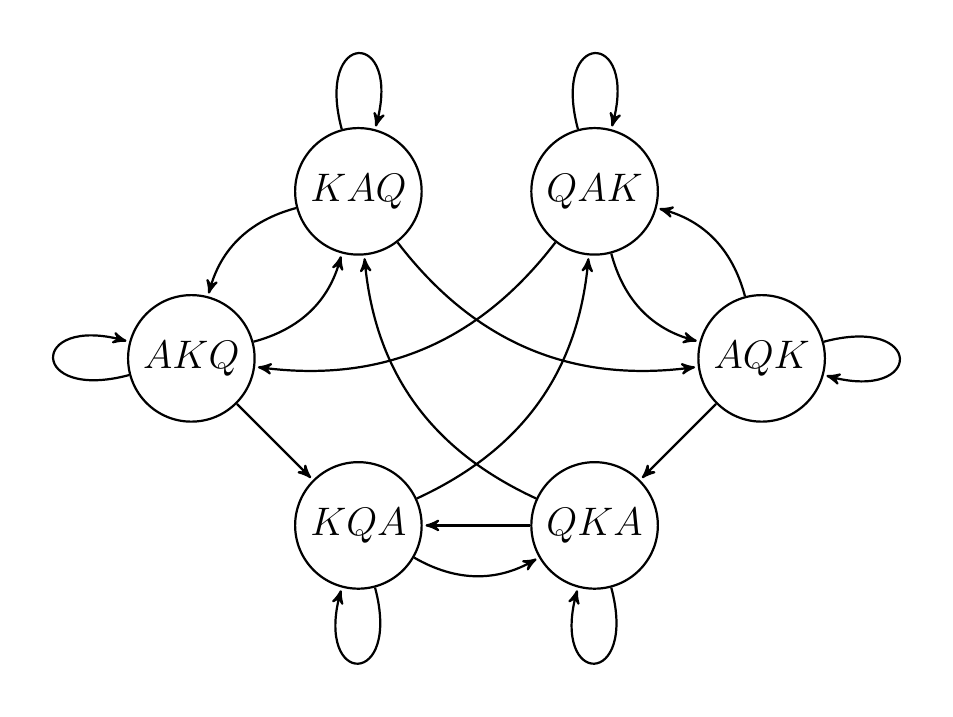
\begin{tikzpicture}[->,>=stealth',shorten >=1pt,auto,node distance=3cm,
                    thick,main node/.style={circle,draw,font=\sffamily\Large\bfseries}]
  \node[main node] (1) {$AKQ$};
  \node[main node] (2) [above right of=1] {$KAQ$};
  \node[main node] (3) [below right of=1] {$KQA$};
  \node[main node] (4) [right of=2] {$QAK$};
  \node[main node] (5) [right of=3] {$QKA$};
  \node[main node] (6) [below right of=4] {$AQK$};


  \path[every node/.style={font=\sffamily\small}]
    (1) edge [bend right=30] node[right]  {} (2)
        edge [left] node[below] {} (3)
        edge [loop left] node[above] {} (1)

    (2) edge [bend right=30] node[above] {} (1)
    edge [bend right=30] node[above] {} (6)
    edge [loop above] node[above] {} (2)

    (3) edge [bend right=30] node[above] {} (4)
    edge [bend right=30] node[below] {} (5)
    edge [loop below] node[below] {} (3)

    (4) edge [bend right=30] node[below] {} (6)
    edge [bend left=30] node[below] {} (1)
    edge [loop above] node[above] {} (4)

    (5) edge [right] node[below] {} (3)
    edge [bend left=30] node[below] {} (2)
    edge [loop below] node[below] {} (5)

    (6) edge [left] node[below] {} (5)
    edge [bend right=30] node[below] {} (4)
    edge [loop right] node[below] {} (6);
\end{tikzpicture}
\end{center}
The graph above represents the markov chain associated with top-in shuffle. All edges have weight $\frac{1}{3}$, and its adjacency matrix gives the one-step transition matrix of this markov process.
\end{example}

\begin{definition} (\textit{Undirected Graph}) Graph of markov chain $G(\mathcal{X})$ is called undirected if $P(x,y)>0 \iff P(y,x)>0$. The exact value of weight doesn't matter, we only care about positivity.
\end{definition}

%/////////////////////////////////////////////////////////////////////////////
\subsection{Basic Properties} 
\begin{definition} (\textit{Irreducible}) $\mathcal{X}$ is called irreducible if (TFAE)
\begin{itemize}
	\item[$\cdot$] $\forall x,y\in \Omega$, $\exists t\in \mathbb{N}$ such that $P^{[t]}(x,y)>0$.
	\item[$\cdot$] The graph $G(\mathcal{X})$ is strongly connected.
\end{itemize}
\end{definition}

\begin{definition} (\textit{Aperiodic}, \textit{Period}) $\mathcal{X}$ is called aperiodic if $\forall x,y\in \Omega$, we have
$$\gcd\{t: P^{[t]}(x,y)>0\}=1$$
For any vertex $x\in \Omega$, define the period of $x$ as $\gcd\{t: P^{[t]}(x,x)>0\}$.
\end{definition}

\begin{lemma} If $\mathcal{X}$ is irreducible, the period of every $x\in \Omega$ is the same. Further, if $G(\mathcal{X})$ is undirected, the period is either $1$ or $2$.
\end{lemma}

\begin{lemma} If $\mathcal{X}$ is irreducible and $G(\mathcal{X})$ is undirected, then $\mathcal{X}$ is aperiodic $\iff$ $G(\mathbf{X})$ is \textit{non-bipartite}. I.e. there is \textbf{Not} a patition $V=V\cup V'$ ($V\cap V' =\emptyset$), such that every edge connects a vertex in $V$ to one in $V'$.
\end{lemma}
\begin{proof} $(\Rightarrow)$ it suffices to show its converse-negative, i.e. bipartite $\Rightarrow$ periodic. Suppose $G(\mathcal{X})$ is bipartite, pick $x,y\in V$ belongs to same side, then every path from $x$ to $y$ requires even \# of steps. So $\gcd\{t: P^{[t]}(x,y)>0\}\geq 2 >1$. \\
$(\Leftarrow)$ Suppose $G(\mathcal{X})$ is bipartite $\iff$ $\exists C\subset G(\mathcal{X})$ is an odd cycle. Pick any $x,y\in \Omega$ and $c\in C$, we can always go through $x\to c\to y$ because the chain is irreducible. Moreover, denote $l(x,y)$ be the path from $x$ to $y$, we can go either
\begin{itemize}
	\item[$\cdot$] $l(x,c)$ $\to$ $C$ $\to$ $l(c,y)$. $t=|l(x,c)|+|C|+|l(c,y)|$
	\item[$\cdot$] $l(x,c)$ $\to$ go on $C$ until the $\frac{|C|-1}{2}$ vertex on $C$, then go back to $c$ $\to$ $l(c,y)$. $t'=|l(x,c)|+|C|-1+|l(c,y)|$
\end{itemize}
We see $\gcd(t,t')$ is already $1$, because they are consecutive integers. So it is aperiodic.
\end{proof}

\begin{lemma} If $\mathcal{X}$ is irreducible, then $\mathcal{X}$ is aperiodic $\iff$ there exists some $t$ such that $P^{[t]}(x,y)>0$ for all $x,y\in \Omega$.
\end{lemma}

\begin{lemma} If $\mathcal{X}$ is irreducible and has at least one self-loop, i.e. $P(x,x)>0$ for some $x$; then $\mathcal{X}$ is aperiodic.
\end{lemma}
\begin{proof} Suppose this loop is on $z$. From $x$ to $y$ we can either
\begin{itemize}
	\item[$\cdot$] $l(x,z)$ $\to$ $l(z,y)$. $t=|l(x,z)|+|l(z,y)|$
	\item[$\cdot$] $l(x,z)$ $\to$ $loop(z)$ $\to$ $l(z,y)$. $t'=|l(x,z)|+1+|l(z,y)|$
\end{itemize}
Same argument as lemma 2.
\end{proof}

%/////////////////////////////////////////////////////////////////////////////
\subsection{Mixing of Markov Chains}
\begin{definition} (\textit{Stationary Distribution}) Let $\mathcal{X}=\{X_t\}$ be a Markov chain. A probability distribution $\pi(\cdot): \Omega\to \mathbb{R}$ over $\Omega$ is a stationary distribution of $\mathcal{X}$ if
$$\bm{\pi}\bm{P}=\bm{\pi}$$
Where $\bm{\pi}$ is $1\times |\Omega|$ vector that stacks the values of $\pi(\cdot)$ together, i.e. $\bm{\pi}=(\pi(x))_{x\in \Omega}$.
\end{definition}

\begin{theorem} (\textit{Ergodic Thm.}) If a Markov chain $\mathcal{X}$ is \textbf{Irreducible} and \textbf{Aperiodic}, then it has a unique stationary distribution $\pi(\cdot)$. In particular
\begin{itemize}
	\item[$\cdot$] $\bm{\pi}$ is the unique left eigenvector of $\bm{P}$ corresponding to eigenvalue $\lambda = 1$.
	\item[$\cdot$] $\lim\limits_{t\rightarrow\infty}P^{[t]}(x,y)=\pi(y)$, $\forall x, y\in\Omega$.
\end{itemize}
\end{theorem}

\begin{definition} (\textit{Reversibility}) Let $\mathcal{X}=\{X_t\}$ be a Markov chain. And $\pi(\cdot): \Omega \to \mathbb{R}$ is a probability distribution over $\Omega$. $\mathcal{X}$ is called reversible with respect to $\pi$ if, for any $x,y\in \Omega$
$$\pi(x)P(x,y)=\pi(y)P(y,x)$$
\textit{Remark.(i)} Intuitively, a markov chain is reversible w.r.t $\pi$ means that the probability mass that flows from note $x \to y$ is same as that from $y \to x$.  \\
\textit{Remark.(ii)} If $\bm{P}$ is symmetric, i.e. $P(x,y)=P(y,x)$, then $\mathcal{X}$ is trivially reversible with respect to uniform distribution on $\Omega$, $\pi(\cdot)\sim U(\Omega)$.
\end{definition}

\begin{lemma} If $\mathcal{X}$ is reversible wrt. $\pi$, then $\pi$ is a stationary distribution of $\mathcal{X}$.
\end{lemma}
\begin{proof} For any fixed $y\in \Omega$:
$$\sum_{x\in\Omega}\pi(x)P(x,y)=\sum_{x\in\Omega}\pi(y)P(y,x)=\pi(y)$$
Implies $\bm{\pi}\bm{P}=\bm{\pi}$.
\end{proof}

\begin{definition} (\textit{Ergodic Flow}) The ergodic flow between nodes $x$ and $y$ wrt. a probability distribution $\pi$ is defined
to be the amount of probability mass flowing between $x,y$:
$$Q(x,y):=\pi(x)P(x,y)=\pi(y)P(y,x)$$
Enables us to write transition probability of reversible markov chain.
\end{definition}

\subsection{Mixing Time and Rate of Convergence}
We hope to construct a metric to capture how statistically ``close'' two distributional objects are from each other.
\begin{definition}(\textit{Total Variation Norm})
For two probability mass function $\pi$, $\mu$, define total variation as
$$\left\|\mu - \pi\right\|_{TV}:=\frac{1}{2}\sum_{x\in \Omega}|\mu(x)-\pi(x)|$$
In particular, if $\mu(\cdot)=P^{[t]}(x_0,\cdot)$ is conditional distribution of deck $\{X_t\}$, given initial deck $x_0$. $\pi(\cdot)=\frac{1}{n!}$, then we define
$$\Delta(t):=\left\|P^{[t]}-\pi\right\|_{TV}=\frac{1}{2}\sum_{x\in \Omega}\left|P^{[t]}(x_0, x)-\frac{1}{n!}\right|$$
\end{definition}

We may apply Monte Carlo simution method, draw large a sample from $P^{[t]}$ (i.e. the deck after $t$ shuffles), then the empirical distribution of sample appoximates $P^{[t]}$. Then, $\Delta(t)$, as a function of $t$, captures the rate by which the Markov chain converges to uniform $\pi(\cdot)$. Moreover, we can set a \textbf{threshold} to $\Delta(t)$ and calculate time needed for the \textbf{deviation of $X_t$ from the limit is bounded by this threshold.}

\begin{definition}(\textit{Mixing Time})
Set the threshold as constant $s$, the time needed is called Mixing Time of Markov chain associated with threshold $s$, given by
$$\tau = \min\left\{t: \Delta(t)\leq s\right\}$$
\end{definition}

Equipped with the metrics and definitions above, we may able to consider the rate in which difference suffling methods (markov chain) converges to stationary distribution, i.e. the uniform distrobution. 




%/////////////////////////////////////////////////////////////////////////////
\section{Types of Shuffles}
%/////////////////////////////////////////////////////////////////////////////
\subsection{Random Transposition}
In the method of random transposition, in each iteration, we pick uniformly at random two cards and switch them. 
\begin{example} (\textit{3-cards Deck Random Transposition}) We still consider our 3-cards deck [AS, KH, QC] and shuffled Random Transposition. Initially $X_0=(\text{AS, KH, QC})$, the first transposition has $\binom{3}{2}=3$ possible cases,
\begin{center}
	\dcards{A}\dcardh{K}\cardc{Q}~~~~\cards{A}\dcardh{K}\dcardc{Q}~~~~\dcards{A}\cardh{K}\dcardc{Q}
\end{center}
And after the first transposition, the deck becomes
\begin{center}
	\cardh{K}\cards{A}\cardc{Q}~~~~\cards{A}\cardc{Q}\cardh{K}~~~~\cardc{Q}\cardh{K}\cards{A}
\end{center}
$G(\mathcal{X})$ is undirect, given by
\begin{center}
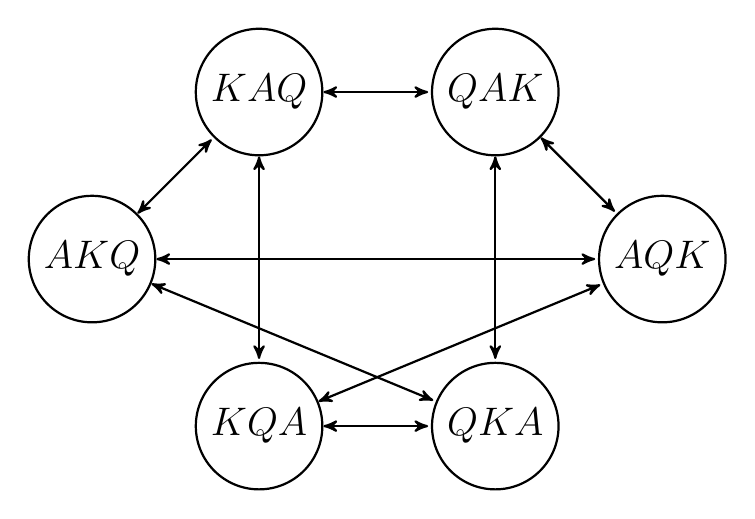
\begin{tikzpicture}[<->,>=stealth',shorten >=1pt,auto,node distance=3cm,
                    thick,main node/.style={circle,draw,font=\sffamily\Large\bfseries}]
  \node[main node] (1) {$AKQ$};
  \node[main node] (2) [above right of=1] {$KAQ$};
  \node[main node] (3) [below right of=1] {$KQA$};
  \node[main node] (4) [right of=2] {$QAK$};
  \node[main node] (5) [right of=3] {$QKA$};
  \node[main node] (6) [below right of=4] {$AQK$};


  \path[every node/.style={font=\sffamily\small}]
    (1) edge [right] node[right]  {} (2)
        edge [left] node[below] {} (5)
        edge [left] node[below] {} (6)

    (2) edge [right] node[right]  {} (3)
    edge [right] node[right]  {} (4)

    (3) edge [right] node[right]  {} (6)
    edge [right] node[right]  {} (5)

    (4) edge [right] node[right]  {} (5)
    edge [right] node[right]  {} (6);

\end{tikzpicture}
\end{center}
\end{example}

\subsection{Riffle Shuffle}
The name Riffle Shuffle refers to the following procedures:
\begin{itemize}
  \item[1.] Split the deck into two parts in each hand.
  \item[2.] Drop the cards one after another to merge into a new deck. The next card is dropped from left hand with probability \# of cards in left hand/\# of cards remaining.
\end{itemize}
\begin{example} (\textit{Riffle Shuffle})  One complete riffle shuffle process is illustrated as below:
\begin{center}
  Input = \cards{A}\cardh{K}\cardc{Q}\cardd{J}\cards{10}\cardh{9}\\
  L: \dcards{A}\cardh{K}\cardc{Q}~~~~R: \cardd{J}\cards{10}\cardh{9} $\xrightarrow{w.p. \frac{1}{2}}$ \cardslot\\
\end{center}

\begin{center}
  L: \dcardh{K}\cardc{Q}~~~~R: \cardd{J}\cards{10}\cardh{9} $\xrightarrow{w.p. \frac{2}{5}}$ \cards{A}\cardslot\\
  L: \cardc{Q}~~~~R: \dcardd{J}\cards{10}\cardh{9} $\xrightarrow{w.p. \frac{3}{4}}$ \cards{A}\cardh{K}\cardslot\\
  L: \dcardc{Q}~~~~R: \cards{10}\cardh{9} $\xrightarrow{w.p. \frac{1}{3}}$ \cards{A}\cardh{K}\cardd{J}\cardslot\\
  \end{center}

\begin{center}
 Output = \cards{A}\cardh{K}\cardd{J}\cardc{Q}\cards{10}\cardh{9}\\
\end{center}
\end{example}


%/////////////////////////////////////////////////////////////////////////////
\section{Simulated Results for Riffle Shuffle}
%/////////////////////////////////////////////////////////////////////////////
It has been shown by Bayer, Diaconis and Persi\cite{bayer} that riffle shuffle has significantly higher rate of convergence, that is, it has short mixing time given a required threshold (distance from output empirical distribution to unifrom distribution.) It is beyond the scope of this project to look into the details of their proofs, instead, we view the result by computer simulation. 

A pure C program is written to finish the shuffling process and compute final distribution (the computation relevent to permutations and the lexicographic orders). The C code is exported to a Python package. It is Python's job to draw the statistics and plots.

\subsection{Mixing of $P^{[t]}$}
The two figures below represents the mixing of $P^{[t]}$. The $x$ axis lists different lexicographic order of permucation instances, when simulating with 4 cards there are $4!=24$ bars, 5 cards deck has $120$ bars. $y$ axis is the counting within totally $100000$ samples. The first subplot depict the outcome after one shuffle, and the sixth subplot is that after 6 shuffles.

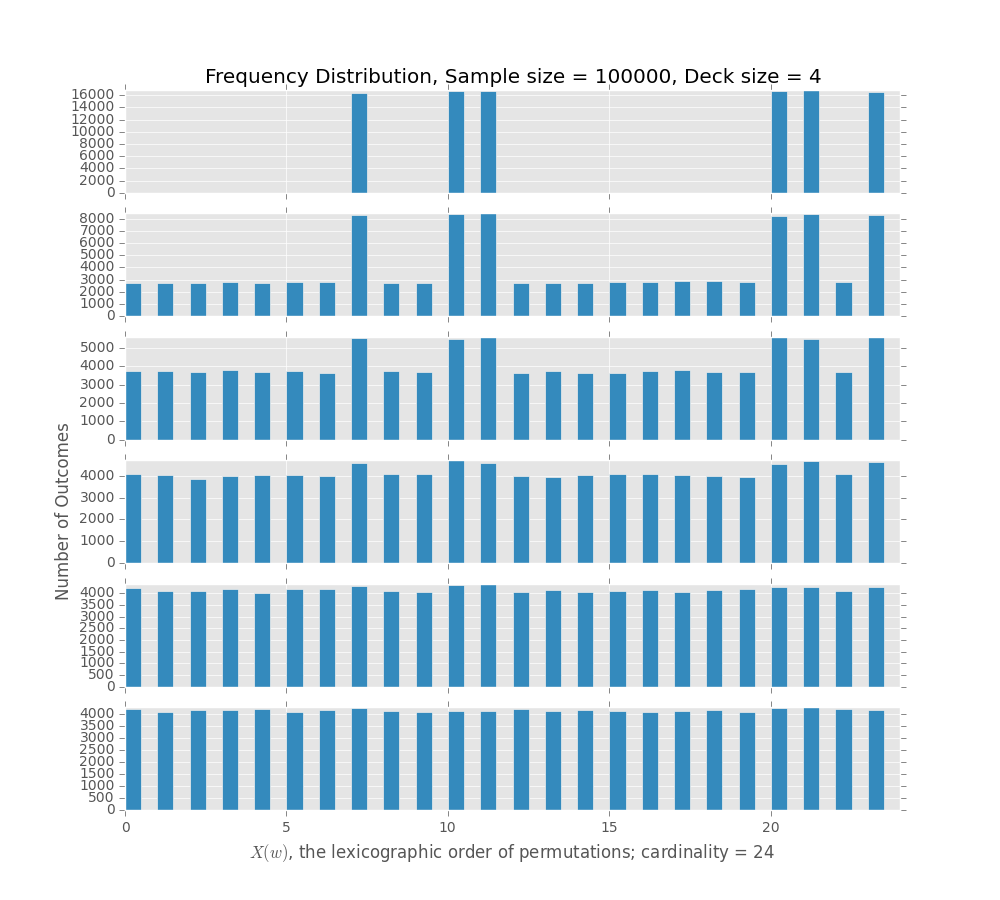
\includegraphics[width=14cm, height=12cm]{figure_2.png}

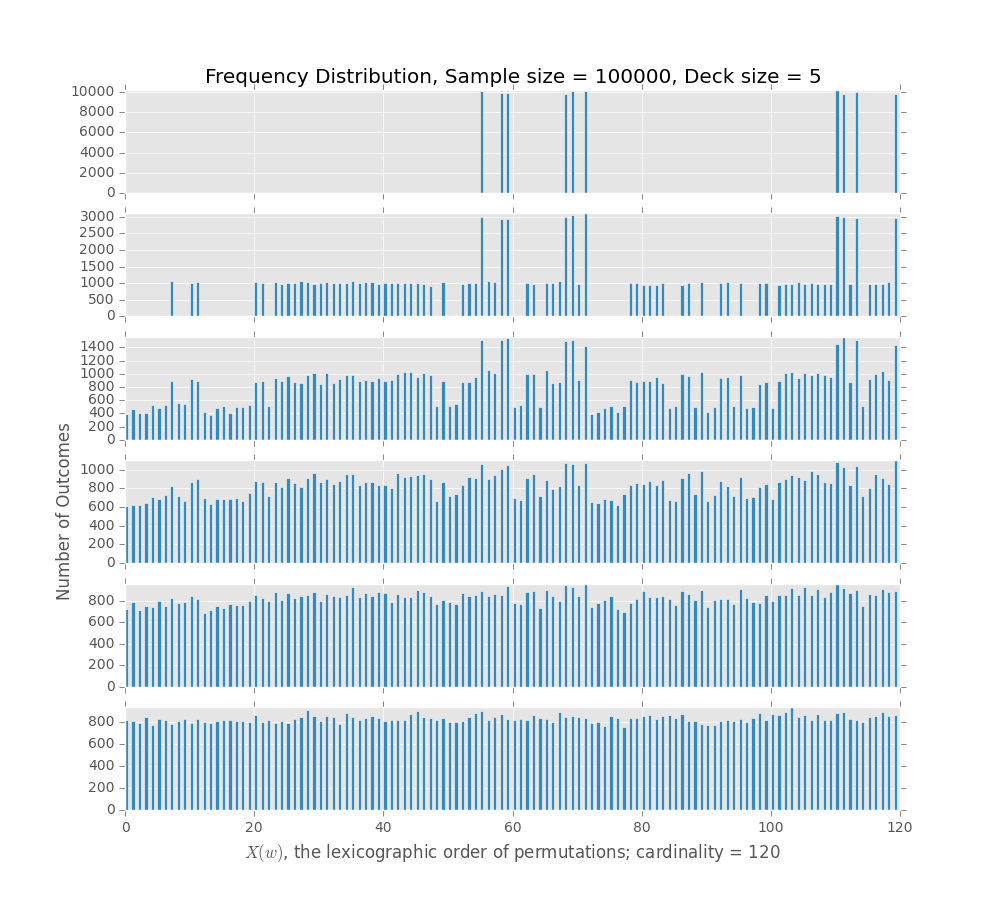
\includegraphics[width=14cm, height=12cm]{figure_3.png}

When deck size $n=6$, there is no space for bars, so we plot the out come in one plot. Lines of different colors represents (unnormalized) pmf after increasing numbers of shuffles.

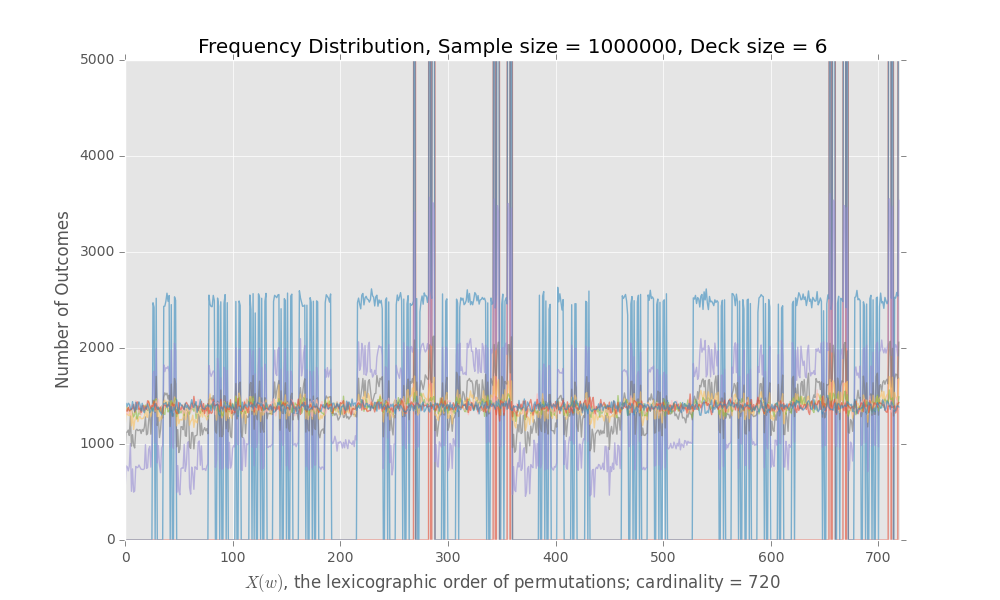
\includegraphics[width=14cm, height=8cm]{figure_4.png}

\subsection{Rate of Convergence}
We now using the simulated data to compute Total Variation Norm from uniform distribution. When choosing a deck $n=6$ cards, shuffle $t$ times for $t=1, 2, ..., 8$, we obtain $\Delta(7)\approx 0.011$, which is fairly close to the targeting distribution.
\begin{center}
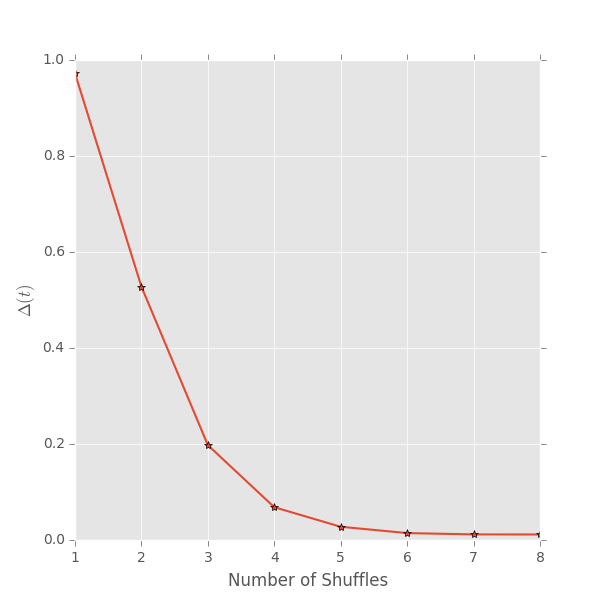
\includegraphics[width=10cm, height=10cm]{figure_5.png}
\end{center}
Hence, with picking appropriate threshold, we can conclude that 6 to 7 riffle shuffles are sufficient to make a 6-cards-deck close enough to as if uniformly distributed in the sense that each permutations arises with equal probability $\frac{1}{n!}$. In fact, due to Bayer and his fellows\cite{bayer}, we still obtain a small quantity (namely 10 to 15) for the number of riffle shuffles required when it comes to a real deck of 52 cards. Since $52!$ is large, simulating this requires heavy computing efforts and optimizion on algorithms, which we leave for further discussion.

\begin{thebibliography}{9}
\bibitem{mit} 
Constantinos Daskalakis: 6.896: Probability and Computation, MIT
\\\texttt{http://people.csail.mit.edu/costis/6896sp11/}

\bibitem{harald} 
Harald Hammarstr\"om.
\textit{Card-Shuffling Analysis with Markov Chains}. 
2005.
 
\bibitem{bayer} 
Bayer, Dave and Diaconis, Persi, 
\textit{Trailing the Dovetail Shuffle to its Lair}. Annals of Applied Probability, 2(2), 294-313, 1992.

\bibitem{mann} 
Brad Mann. 
\textit{How many times should you shuffle a deck of cards}. 
Topics in Contemporary Probability and Its Applications, Harvard University, 1995.

\bibitem{ross} 
Sheldon M. Ross.
\textit{Introduction to Probability Models, Eleventh Edition}. ISBN: 978-0-12-407948-9, 2015

\end{thebibliography}





\end{document}